%% Преамбула TeX-файла

% 1. Стиль и язык
\documentclass[utf8x, 14pt]{G7-32} % Стиль (по умолчанию будет 14pt)

% Остальные стандартные настройки убраны в preamble.inc.tex.
\include{preamble.inc}

% Настройки листингов.
\ifPDFTeX
\include{listings.inc}
\else
\usepackage{local-minted}
\fi

% Доп определения
\newcommand{\R}{\mathbb{R}}
\usepackage{subcaption}

% Полезные макросы листингов.
\include{macros.inc}
% Стиль титульного листа и заголовки
% \include{00-title}


\begin{document}

\frontmatter % выключает нумерацию ВСЕГО; здесь начинаются ненумерованные главы: реферат, введение, глоссарий, сокращения и прочее.

% \maketitle %создает титульную страницу





%\listoffigures                         % Список рисунков

%\listoftables                          % Список таблиц

%\NormRefs % Нормативные ссылки
% Команды \breakingbeforechapters и \nonbreakingbeforechapters
% управляют разрывом страницы перед главами.
% По-умолчанию страница разрывается.

% \nobreakingbeforechapters
% \breakingbeforechapters

% \include{00-abstract}

\tableofcontents

\printnomenclature % Автоматический список сокращений

\Introduction

За последние 10 лет большое распространение в промышленности получили манипуляционные роботы, способные решать большой спектр задач, начиная от перемещения объектов и механической обработки деталей, заканчивая сортировкой и дефектоскопией. Исследования в области силомоментного управления в период 70---90-ы гг. прошлого века позволили использовать манипуляционных роботов в задачах, где важно соблюдение технологического процесса с заданными показателями точности к усилию и импульсу, которые сообщаются объектам манипулирования или обрабатываемым деталям. Так появились два класса алгоритмов силомоментного управления: непрямые и прямые \cite{Handbook}. Оба этих метода актуальны и сегодня, каждый из них имеет свои особенности и сферы применения. В данный период многими знаменитыми учеными были изучены, а также сформулированы и описаны методы силомоментного управления \cite{Khatib1986_force_control, Villani2016, Salisbury1980, Yoshikawa1987, RaibertMH;Craig2015}. С 1990 по 2010 в связи с повышением спроса со стороны промышленной индустрии \cite{Yamada1995, Handbook, Yoshikawa1990} на согласованное использование нескольких манипуляторов в общем рабочем пространстве было проведено большое количество исследований алгоритмов кооперативного управления манипуляторами. Актуальность вопроса была также обусловлена необходимостью разработки математического аппарата для унификации синтеза алгоритмов схватывания, энергетически оптимального, а также адаптивного к форме объекта манипулирования \cite{Takahashi2008,Yoshikawa1991, Park1989}.\\

В последнее двадцатилетие появилась высокая потребность в алгоритмах кооперативного управления не только многопалыми схватами, но и промышленными манипуляторами. Тенденции к развитию были сформированы благодаря распространению антропоморфных роботов, имеющих большой потенциал выполнять координационно достаточно сложную работу, подобно человеку. На сегодняшний день антропоморфные роботы стали примером концепции создания роботов, пригодных для функционирования в среде человека, тем самым дав дорогу для развития коллаборативной робототехники.

\begin{figure}[ht]
  \centering
  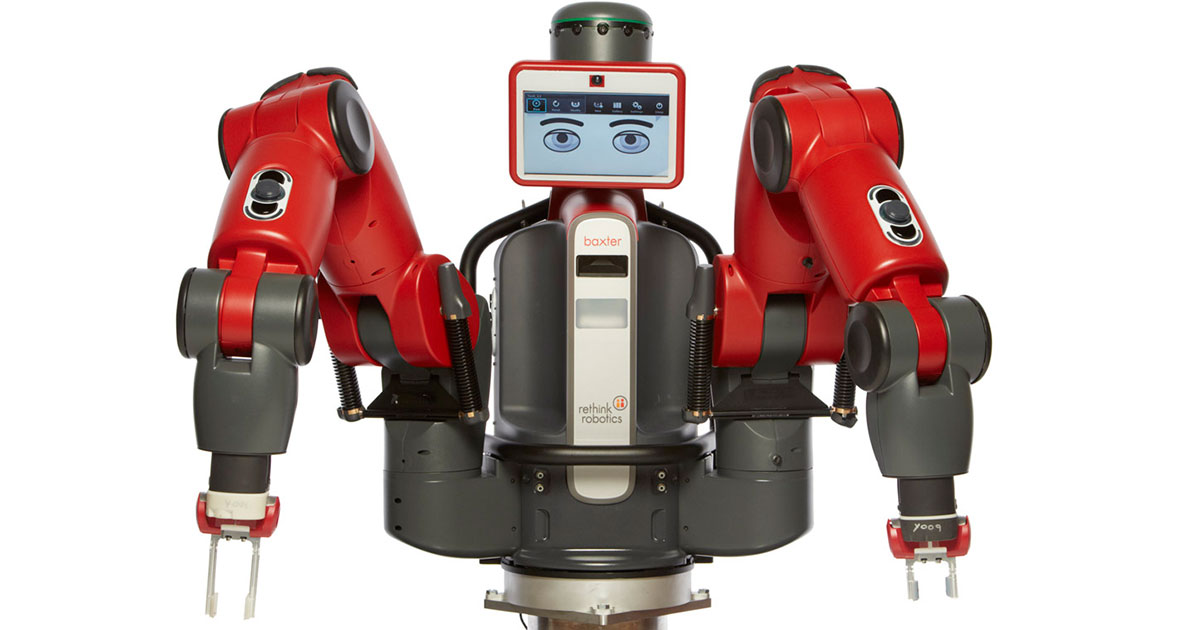
\includegraphics[height=0.45\textwidth]{inc/img/baxter}
  \caption{Антропоморфный робот \textit{Baxter}}
  \label{fig:baxter}
\end{figure}

Как отмечалось ранее, использование двух и более манипуляционных роботов в составе антропоморфного робота(рисунок \ref{fig:baxter}) позволяет совершать более сложные операции над объектом манипулирования. Кроме того, существует несколько других факторов, мотивирующих к использованию кооперации манипуляционных роботов:
\begin{itemize}
  \item \textbf{Сходство с человеком:} большое колличество коллаборативных роботов, в особенности домашние помощники и роботы, использующиеся в медицине, в частности в хирургии, адаптированы для взаимодействия с человеком и телеуправления посредством рук человека. Это дает возможность использовать эволюционно приобретенные человеческие навыки координации и манипулирования объектами в алгоритмах управления роботами \cite{coop_manipulator_survey};
  \item \textbf{Гибкость:}использование двух и более манипуляционных роботов позволяет получить большее колличество конфигураций благодаря увеличенному числу степеней подвижности. Это позволяет выполнять операции более энергоэфективно \cite{Ajoudani2017} или точно \cite{Faroni2016};
  \item \textbf{Грузоподъемность:} кооперация из манипуляторов может выполнять манипулирование объектами массой в разы большей, чем может поднять манипуляционный робот в одиночку \cite{AzizZadeh2019};
\end{itemize}

 Сейчас кооперативное управление можно разделить на два больших класса \cite{coop_manipulator_survey}: нескоординированное и скоординированное. Скоординированное управление можно также разделить на два типа: синхронизированное и бимануальное. Первое решает проблему планирования путей и траекторий для согласованного (без столкновений) движения нескольких манипуляторов. Второе же рассматривает несколько манипуляционных роботов как мультиагентную систему, каждый агент в которой принимает участие в выполнении одной общей для всех задачи. Кооперативная система манипуляционных роботов имеет большее число переменных состояния чем независимые роботы. Эти переменные состояния зачастую необходимы для управления, например контактное усилие, для удерживания предметов двумя роботами.

В связи с возросшим интересом к системам из двух и более манипуляционных роботов большую востребованность получили методы кооперативного управления манипуляторами, позволяющие выполнять такие задачи, как сборка деталей \cite{Sun2002}, механическая обработка деталей \cite{AzizZadeh2019}, удержание и позиционирование гибких и подвижных объектов \cite{Pfeffer1993} с заданными показателями качества управления. Разрабатываемый алгоритм кооперативного управления может быть использован в системах управления домашними роботами-помощниками, коллаборативными роботами, экзоскелетов, промышленных роботов, осуществляющих манипулирование тяжелыми объектами с высокой гибкостью реконфигурирования производства.

Для разработки алгоритма кооперативного управления в рамках данной работы ставятся следующие задачи:
\begin{enumerate}
  \item провести  обзор  литературных  источников,  рассматривающих  алгоритмы  гибридного позиционного/силомоментного  управления  для  одного  и  нескольких  артикулированных манипуляционных  роботов  за  последние  10  лет,  выделить  основные  методы,  описать  их достоинства   и   недостатки.   Обосновать   актуальность   рассматриваемой   задачи,
  \item рассмотреть   динамическую   и   кинематическую   модель   двух   артикулированных манипуляционных  роботов,  жестко  удерживающих  объект  в  заданных  точках  контакта. Масса и  вектор центра  масс объекта  считаются неизвестными.  Параметры  динамической модели  каждого  робота-манипулятора,  осуществляющего  манипулирование  объектом, считаются  известными.  Доступными  сигналами  для  управления  являются  моменты  на сочленениях каждого робота-манипулятора. Измеряемыми сигналами являются положение и  скорости  сочленений,  моменты  на  сочленениях,  а  также  силы  и  моменты  с датчиков, установленных   на   рабочем   инструменте   каждого   манипулятора,
  \item синтезировать   алгоритм   гибридного   силомоментного/позиционного   управления   для математической    модели    двух    артикулированных    манипуляционных    роботов, удерживающих объект, адаптивный к параметрической неопределенности модели объекта манипулирования,  обеспечивающий  статическую  ошибку  между  желаемыми  и  текущими положениями в рабочем пространстве не более 10 мм, силами и моментами действующимина  объект  манипулирования  не  более  20Н/50Нм  при  условии  наличия  полного  ранга матрицы  Якоби,  а  также  при  отсутствии  помех  измерений,  неучтенных  внешних  и параметрических  возмущений,
  \item провести  численное  моделирование  предложенного алгоритма  в  задаче  удерживании  заданного  постоянного  усилия  манипулируемым обьектом, с сохранением заданного положения.
\end{enumerate}






% Целью работы является создание всякой всячины. Для достижения поставленной цели необходимо решить следующие задачи:
%
% \begin{itemize}
% \item проанализировать существующую всячину;
% \item спроектировать свою, новую всячину;
% \item изготовить всякую всячину;
% \item проверить её работоспособность.
% \end{itemize}
%
% Проверяем как у нас работают сокращения, обозначения и определения "---
% MAX,
% \Abbrev{MAX}{Maximum ""--- максимальное значение параметра}
% API
% \Abbrev{API}{application programming interface ""--- внешний интерфейс взаимодействия с приложением}
% с обратным прокси.
% \Define{Обратный прокси}{тип прокси-сервера, который ретранслирует}


\mainmatter % это включает нумерацию глав и секций в документе ниже

\chapter{Аналитический обзор алгоритмов одиночного и кооперативного силомоментного управления}
\label{cha:analysis}
%
% % В начале раздела  можно напомнить его цель
%

Для манипулирования объектами порой не достаточно стандартного позиционного управления. Использование силомоментного управления позволяет решать следующие прикладные задачи:
\begin{itemize}
  \item сборка деталей,
  \item вставка детали в отверстие,
  \item полировка/шлифовка или фрезерование с заданным усилием,
  \item вкручивание винтов.
\end{itemize}

Для синтеза любого алгоритма силомоментного управления зачастую необходимо знание динамической модели манипулятора. Модель манипулятора описываемая классическим уравнением нелинейной системы, которое может быть получена из уравнения Эйлера-Лагранжа:
\begin{equation}
  M(q)\ddot{q} + C(q,\dot{q})\dot{q} + g(q) = \tau - J^\top f_{ext},
  \label{eq:base_one_manipulator_model}
\end{equation}
где $q, \dot{q}, \ddot{q} \in \R_{n\times1}$ --- обобщенные положения, скорости и ускорения в сочленениях, $\tau \in \R_{n \times 1}$ --- момент на сочленениях манипулятора, управляющий сигнал, $J \in \R_{6 \times n}$ --- геометрическая матрица Якоби манипулятора, $f_{ext} \in \R_{n\times1}$ --- силы, действующие на рабочий инструмент, вызванные внешним возмещением, $M(\cdot )\in \R_{n\times n}$ --- матрица инерции, $C(\cdot ) \in \R_{n\times n}$ --- матрица Кориолисовых и центробежных сил, $g(\cdot ) \in \R_{n\times 1}$ --- матрица гравитационных сил, $n$ --- число звеньев манипулятора.

\section{Алгоритмы одиночного силомоментного управления}

Алгоритмы силомоментного управления одним манипулятором впервые были разработаны и описаны в работах таких исследователей, как: Б. Сицилиано, Н. Хогана, Р. Бонитц, Т. Йошикава, У. Хатиба. Эти методы могут быть разделены на прямые и непрямые \cite{Handbook}. Прямые методы используют обратную связь по силе на рабочем инструменте, для непрямых обратная связь по силе не нужна. При этом первые представляют из себя стратегию поддатливого внешним силам позиционного управления, вторые же напротив робастны к заданным направлениям внешних сил и адаптивны к другим. Наибольшее развитие с 90-х годов получили методы прямого силомоментного управления, благодаря их высокой востребованности в индустриальной робототехнике, устанавливающей высокие требования к соблюдению технологического процесса процесса \cite{Ha1999}. Однако, сейчас новый виток популярности получили непрямые методы силомоментного управления благодаря работам Стефано Страмиджоли и его коллег в области коллаборативного управления манипуляционными роботами. Данные методы основываются на информации о внутренней энергии системы \cite{StarmidgoliImpedanceControl}, \cite{StarmidgoliImpedanceControl2} и имеют большой потенциал в задачах, где необходимо безопасное взаимодействие робота и человека. Основной нюанс данных методов --- отсутствие возможности управления желаемым усилием и соответственно отсутствие необходимости измерения усилия, что делает непрямые методы силомомного управления эффективными в задачах, где необходима податливость и адаптивность к воздействиям внешней среды, но абсолютно неприменимы в задачах где необходима робастность к ним \cite{indirect_to_direct}.\\

\begin{figure}
  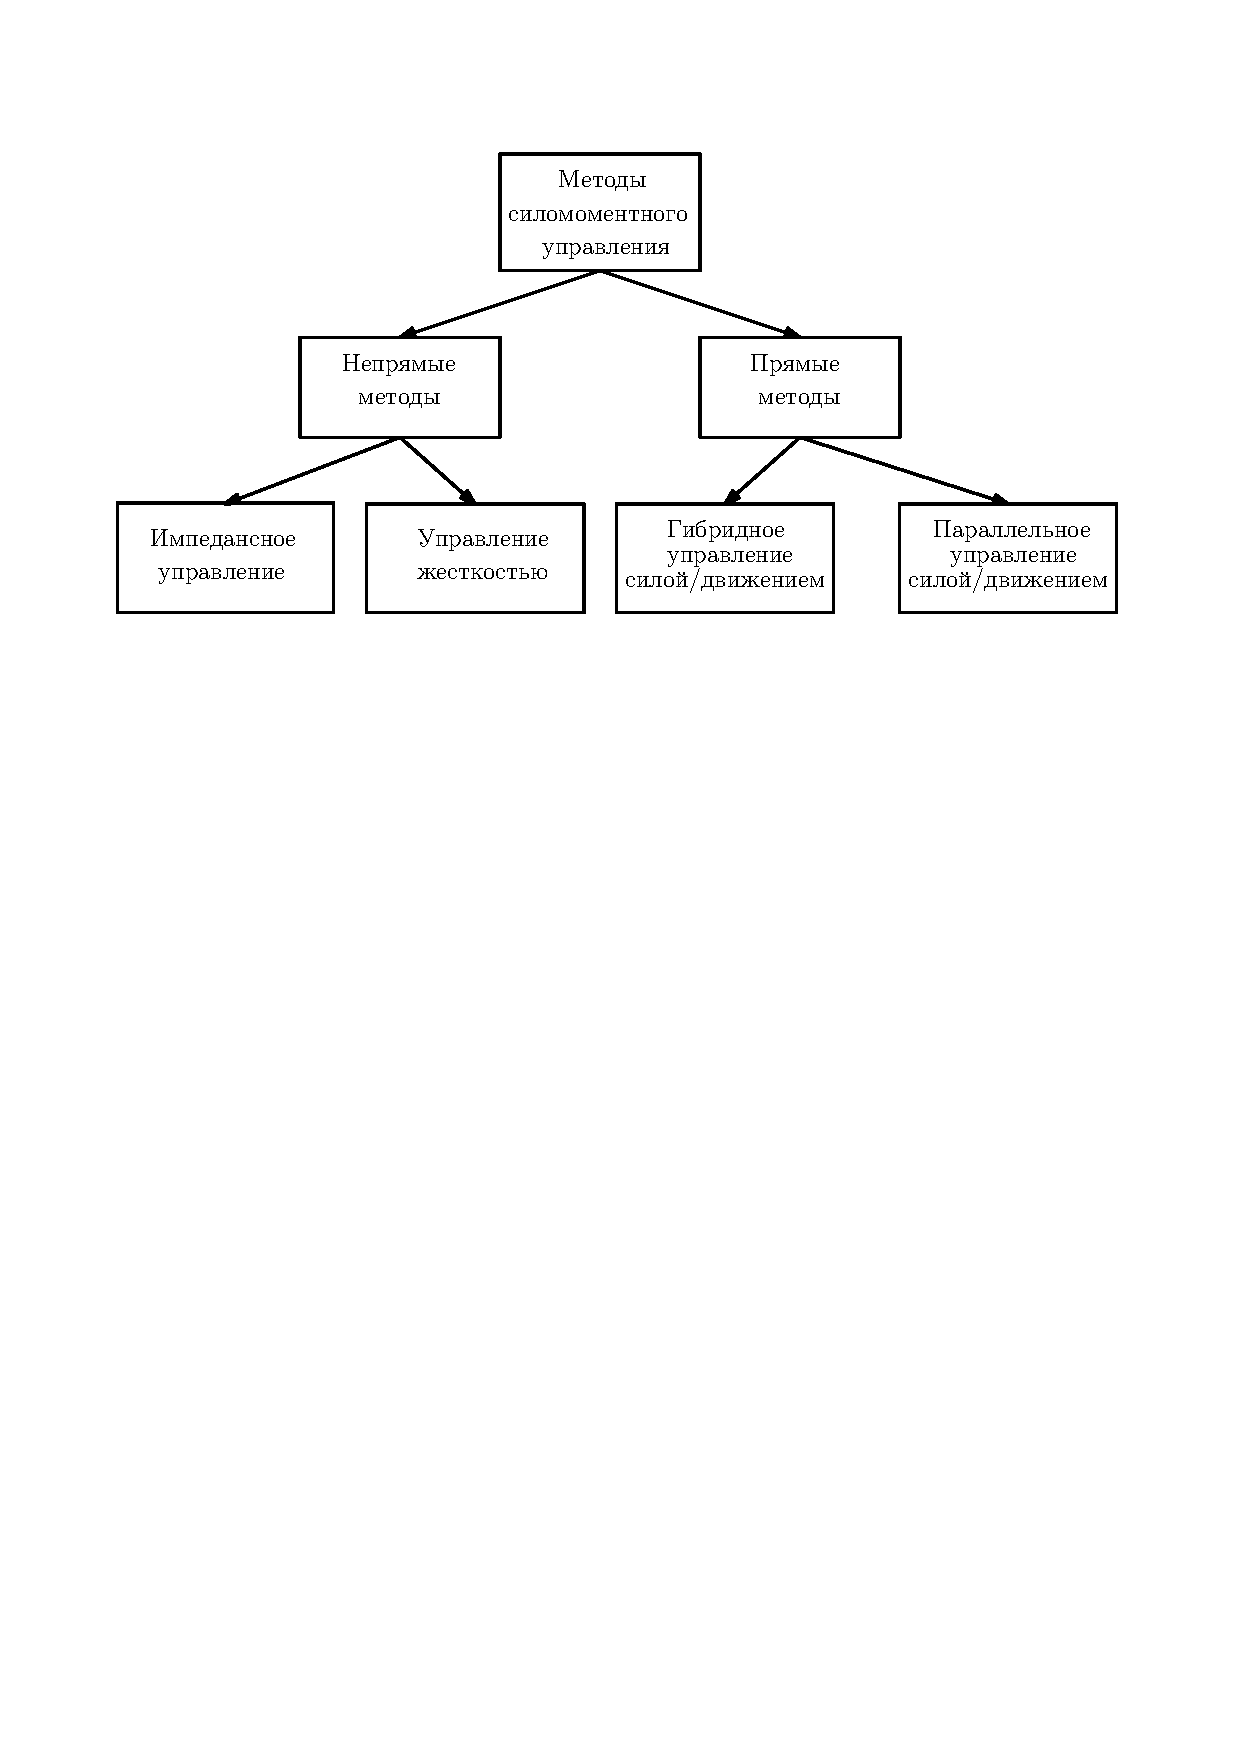
\includegraphics[width=\textwidth]{inc/img/force_control_methods}
  \caption{Методы силомоментного управления}
  \label{split_fs_control}
\end{figure}

Все методы силомоментного управления применимы для управления и в операционном и в конфигурационном пространствах. Выбор того или иного метода и пространства описания алгоритма управления происходит исходя из требований к точности и желаемой реакции системы на внешнее возмущение.
\subsection{Управление жесткостью}
Классически, управление жесткостью подразумевает виртуальное взаимодействие манипулятора с объектами окружения по закону Гука \cite{Siciliano2000} в конфигурационном или операционном  пространстве с компенсацией гравитации и демпфированием:
\begin{align}
  \tau &= Kp_{j}\cdot  \delta q + Kd_{j}\dot{q} + g(q), \quad \delta q = (q^* - q),   \label{eq:stiffnes_base_1}\\
  f &= Kp_{e}\cdot \delta p + Ke_{j}\dot{p} + g_e(q), \quad \delta p = (p^* - p), \label{eq:stiffnes_base_2}
\end{align}
где $f \in \R_{6 \times 1}$ --- вектор сил/моментов, действующих на рабочий инструмент, $p \in \R_{6 \times 1} = \displaystyle \begin{bmatrix} x& y& z& \phi& \theta& \psi& \end{bmatrix}^\top$ --- вектор положения и ориентации (углы Эйлера) рабочего инструмента в базовой системы координат, $q \in \R_{n \times1}$ --- вектор обобщенных координат, положений сочленений, $Kp_{e} \in \R_{6 \times 6},\ Kp_{j} \in \R_{n \times n}$ --- матрицы жесткости (обычно диагональные), описывающие виртуальные упругие связи в операционном и конфигурационном пространстве соответственно, $Kd_{e} \in \R_{6 \times 6},\ Kd_{j} \in \R_{n \times n}$ --- соответствующие матрицы демпфирования (обычно диагональные), $g_e(q) \in \R_{6 \times 1}$ --- вектор гравитационных сил модели манипулятора в операционном пространстве.\\

Из принципа виртуальной работы и виртуальных перемещений \cite{Spong2006} следует, что между вектором сил/моментов и вектором моментов на сочленениях существует геометрическое соотношение в виде матрицы Якоби:
\begin{equation}
  \tau = J^\top f, \qquad  f =\begin{bmatrix} f_x& f_y & f_z & m_x & m_y & m_z\end{bmatrix}^\top.
  \label{eq:Tvsf}
\end{equation}

Стоит отметить, что между скоростями в операционном пространстве и конфигурационном пространстве также существует взаимосвязь \cite{Handbook}:
\begin{equation}
  \delta p = J_a \delta q,
  \label{eq:Ja_def}
\end{equation}
где $J_a \in \R_{6 \times n}$ --- аналитическая матрица Якоби манипулятора: $J_a = \dfrac{\partial p}{\partial q}$.\\

Из \eqref{eq:Tvsf},\eqref{eq:stiffnes_base_2} и \eqref{eq:Ja_def} следует, что между матрицами жесткости, в конфигурационном и операционном пространствах существует взаимосвязь:
\begin{equation}
  \tau = J^\top Kp_{e}J_a \delta q + J^\top Kd_e J_a\dot{q} + J^\top g_e(q),\qquad \begin{cases}
    Kp_{j} = J^\top Kp_{e}J_a,\\
    Kd_{j} = J^\top Kd_{e}J_a.
  \end{cases}
  \label{eq:stiffnes_matrix_dep}
\end{equation}

От аналитической матрицы Якоби к геометрической можно перейти следующим образом \cite{Spong2006}:
\begin{equation}
  J_a = T_a^{-1} J,\  T_a = \begin{bmatrix} I & 0 \\ 0 &  B(\alpha) \end{bmatrix}, B(\alpha) = \begin{bmatrix} cos(\psi)sin(\theta) & -sin(\psi) & 0 \\ sin(\psi)sin(\theta) & cos(\psi) & 0\\ cos(\theta) & 0 & 1 \end{bmatrix}.
  \label{eq:JavsJ}
\end{equation}
Тогда подставляя \eqref{eq:JavsJ} в \eqref{eq:stiffnes_matrix_dep}, получим:
\begin{equation}
  Kp_{j} = J^\top Kp_{e} T_a^{-1} J, \qquad Kd_{j} = J^\top Kd_{e} T_a^{-1} J.
  \label{eq:stiffnes_matrix_dep_final}
\end{equation}

\subsection{Импедансное управление}
Классическое управление жесткостью не гарантирует схождения ошибки управления к нулю при ненулевой скорости перемещения \cite{indirect_to_direct}. Дело в том, что рассмотренный линейный алгоритм управления не компенсирует нелинейную динамику в виде Кориолисовых и центробежных сил, а потому такой подход работает только на малых скоростях  $\dot{q}(t)$. Данная проблема была решена в предложенном  алгоритме управления \cite{Yoshikawa2000}, в котором  взаимодействие робота и среды описывается <<виртуальной>> системой масса-пружина-демпфер. Обеспечить асимптотическую устойчивость системы позволила линеаризация обратной связью с компенсацией всей динамики, представляющая из себя внутренний контур управления.\\

Импедансное управление также, как и управление жесткостью может быть описано, как для операционного, так и для конфигурационного пространства.
\paragraph{Конфигурационное пространство} Внутренний контур данного алгоритма описывается следующим уравнением, позволяющим линеаризовать объект управления:
\begin{equation}
   \tau = M(q)u_l + C(q,\dot{q})\dot{q} + g(q) + J^\top f_{ext},
   \label{eq:lin_fb_init}
\end{equation}
где $u_l$ --- сигнал управления внешним контуром. При подстановке  \eqref{eq:lin_fb_init} в \eqref{eq:base_one_manipulator_model} получим линейную систему:
\begin{equation}
  \ddot{q} = u_l.
  \label{eq:lin_fb_res}
\end{equation}

\begin{figure}
  \centering
  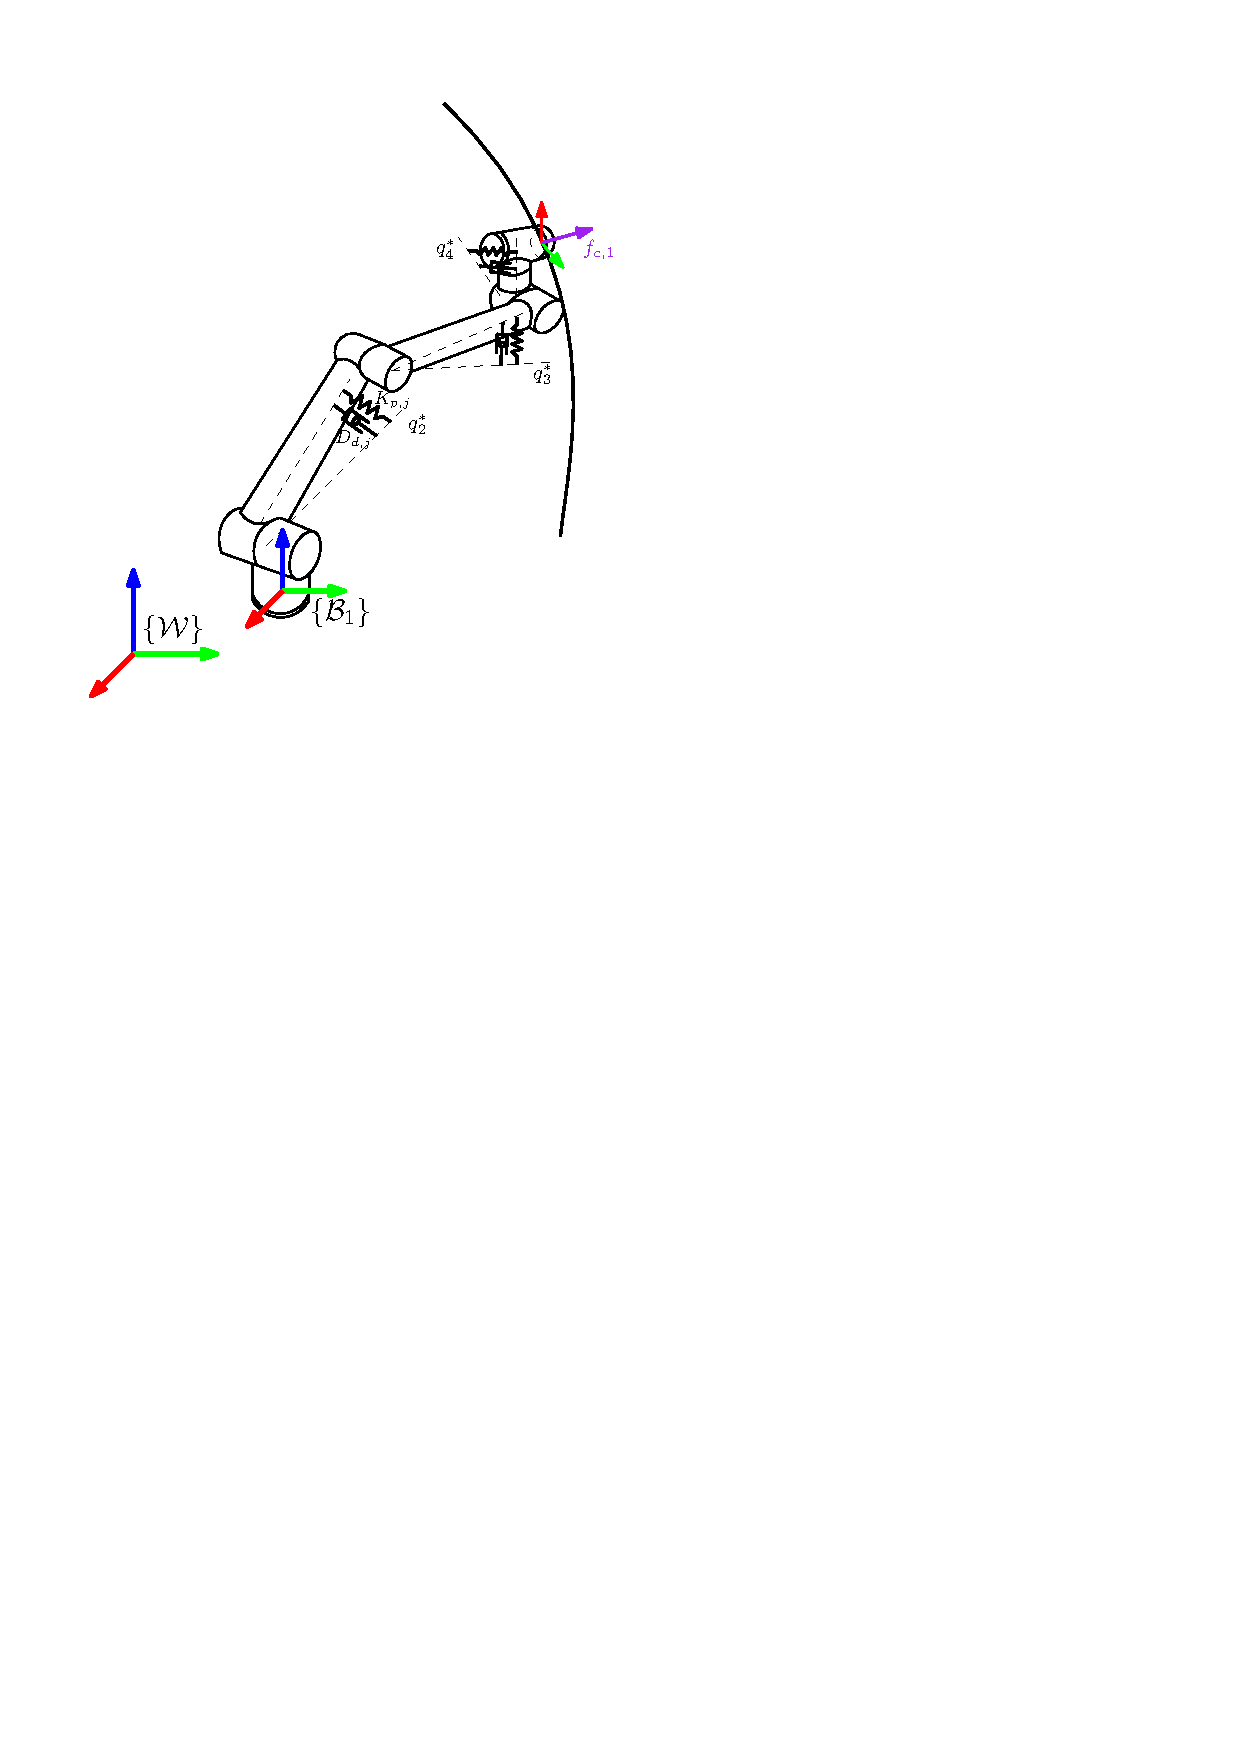
\includegraphics[width=0.6\textwidth]{inc/img/coop_impedance}
  \caption{Импедансное управление в конфигурационном пространстве}
  \label{fig:js_impedance}
\end{figure}
Систему масса-пружина-демпфер в конфигурационном пространстве (рисунок \ref{fig:js_impedance}) можно описать следующим дифференциальным уравнением:
\begin{equation}
  \tau_{ext} = J^\top f_{ext}  = M_{d,j}(\ddot{q}^* - \ddot{q}) +  D_{d,j} (\dot{q}^* - \dot{q}) + K_{d,j} (q^* - q)
  \label{eq:impedance_ref}
\end{equation}
Тогда, подставив \eqref{eq:impedance_ref} в \eqref{eq:lin_fb_res}, получим финальное выражение для внешнего контура:
\begin{align}
  u_{l} = \ddot{q}^* +   M_{d,j}^{-1}\left[ D_{d,j}(\dot{q}^* - \dot{q}) + K_{d,j} (q^* - q) - \tau_{ext} \right]
  \label{eq:impedance_mathing}
\end{align}
Скомпануем уравнение внутреннего контура \eqref{eq:lin_fb_init} и внешнего \eqref{eq:impedance_mathing}:
\begin{equation*}
  \begin{split}
    \tau = M(q) \left[ \ddot{q}^* + M_{d,j}^{-1}\left( D_{d,j}(\dot{q}^* - \dot{q}) + K_{d,j} (q^* - q) - \tau_{ext} \right) \right] + C(q,\dot{q})\dot{q}  +\\
     + g(q) + J^\top f_{ext} = M(q)\ddot{q}^* + M(q)M_{d,j}^{-1}\left( D_{d,j}(\dot{q}^* - \dot{q}) + K_{d,j} (q^* - q)\right) - \\
     - M(q)M_{d,j}^{-1}\tau_{ext} + C(q,\dot{q})\dot{q} + g(q) + \tau_{ext}
  \end{split}
\end{equation*}
Итоговое выражение будет иметь следующий вид:
\begin{equation}
  \begin{split}
    \tau = M(q)\ddot{q}^* + M(q)M_{d,j}^{-1}\left[ D_{d,j}(\dot{q}^* - \dot{q}) + K_{d,j} (q^* - q)\right] + C(q,\dot{q})\dot{q} +\\
      \quad + g(q) + \left(I - M(q)M_{d,j}^{-1}\right)\tau_{ext}
  \end{split}
  \label{eq:impedance_final}
\end{equation}
Стоит отметить, что в данной версии импедансного управления необходима обратная связь по силе $f_{ext}$ или моментам $\tau_{ext}$. Однако, обратную связь по силе можно и не использовать, если представить, что среда имеет те же инерционные параметры, что и сам манипулятор, т.е $M_{d,j} = M(q)$:
\begin{equation}
  \begin{split}
    \tau = M(q)\ddot{q}^* + \left[ D_{d,j}(\dot{q}^* - \dot{q}) + K_{d,j} (q^* - q)\right] +\\
     + C(q,\dot{q})\dot{q} + g(q)
  \end{split}
  \label{eq:impedance_without_fs}
\end{equation}


\paragraph{Операционное пространство}
Аналогично конфигурационному пространству импедансное управление в операционном пространстве представляется в следующем виде \cite{Yoshikawa2000}:
\begin{equation}
   J^{-T}\tau = M_e(q)u_l + C_e(q,\dot{q})\dot{p} + g_e(q) + f_{ext},
   \label{eq:cart_lin_fb_init}
\end{equation}
где $M_e(q) = J^{-\top} M(q) J^{-1}$ --- матрица инерции модели манипулятора в операционном пространстве, $C_e(q, \dot{q}) = J^{-\top} C(q,\dot{q}) J^{-1} - M_e(q) \dot{J} J^{-1}$ --- матрица Кориолисовых и центробежных сил модели манипулятора в операционном пространстве, $g_e(q) = J^{-\top} g(q)$ --- матрица Кориолисовых и центробежных сил модели манипулятора в операционном пространстве.

При подстановке  \eqref{eq:cart_lin_fb_init} в \eqref{eq:base_one_manipulator_model} получим линейную систему:
\begin{equation}
  \ddot{p} = u_l
  \label{eq:cart_lin_fb_res}
\end{equation}
\begin{figure}[ht]
  \centering
  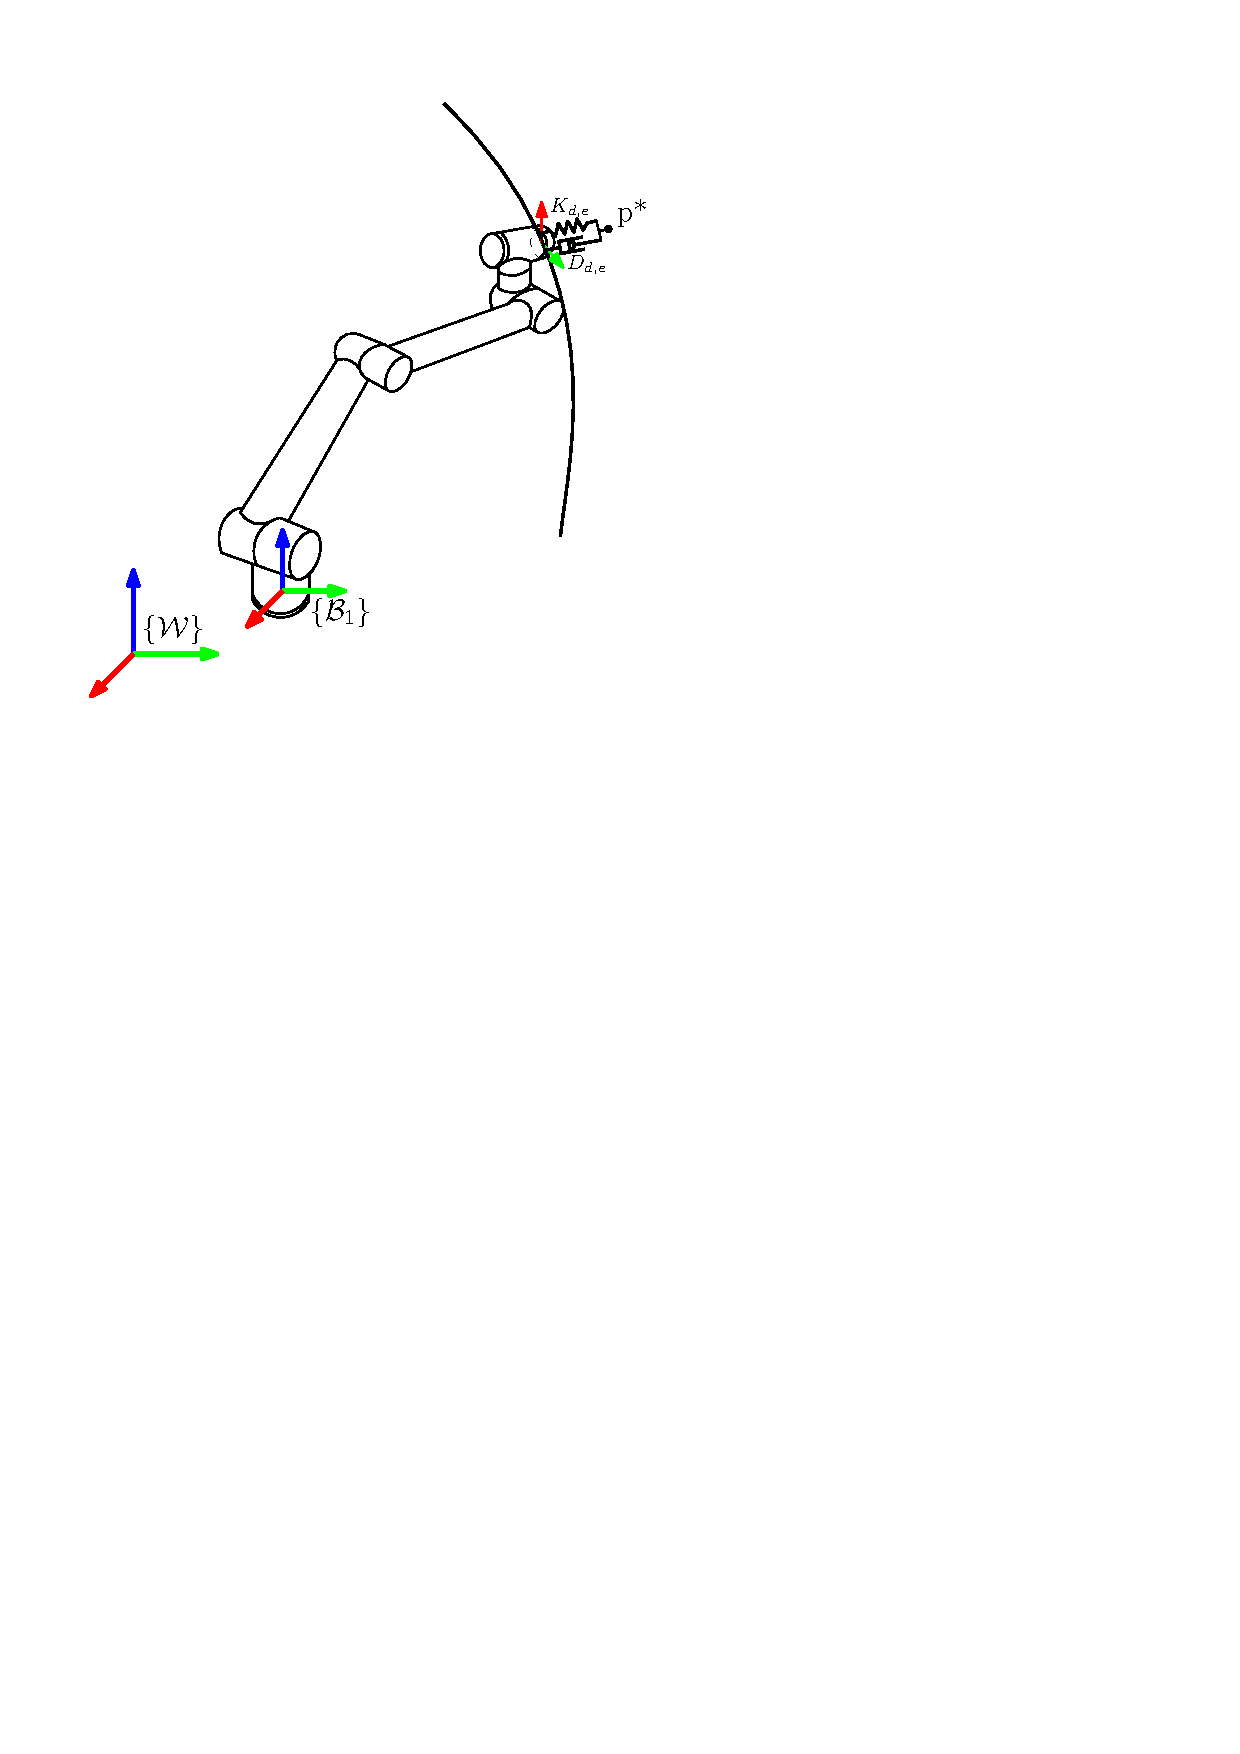
\includegraphics[width=0.6\textwidth]{inc/img/coop_impedance_cart}
  \caption{Импедансное управление в операционном пространстве}
  \label{fig:os_impedance}
\end{figure}

Для операционного пространства желаемое поведение при контакте, повторяющее поведение системы масса-пружина-демпфер (рисунок \ref{fig:os_impedance}) описывается следующим выражением:
\begin{equation}
  f_{ext} = J^{-\top} \tau_{ext}  = M_{d,e}(\ddot{p}^* - \ddot{p}) +  D_{d,e} (\dot{p}^* - \dot{p}) + K_{d,e} (p^* - p).
  \label{eq:cart_impedance_ref}
\end{equation}
Выполняя преобразования аналогично предыдущему параграфу, получим:
\begin{equation}
  \begin{split}
    \tau = M_e(q)\ddot{p}^* + M_e(q)M_{d,e}^{-1}\left[ D_{d,e}(\dot{p}^* - \dot{p}) + K_{d,e} (p^* - p)\right]+ \\
      \quad+ C_e(q,\dot{q})\dot{p} + g_e(q) + \left(I - M(q)M_{d,e}^{-1}\right)f_{ext}.
  \end{split}
  \label{eq:cart_impedance_final}
\end{equation}
Для $M_{d,e} = M_e(q)$:
\begin{equation}
  \begin{split}
    \tau = M_e(q)\ddot{p}^* + \left[ D_{d,e}(\dot{p}^* - \dot{p}) + K_{d,e} (p^* - p)\right] + C_e(q,\dot{q})\dot{p} + g_e(q).
  \end{split}
  \label{eq:cart_impedance_without_fs}
\end{equation}

\subsection{Гибридное управление}
Гибридное управление позволяет разделить позиционное управление и силомоментное на компоненты, что позволяет выполнять перемещение по заданной траектории на поверхности, с поддержанием желаемого усилия по осям, ортогональным к ней \cite{Handbook}.
\begin{equation}
  \begin{cases}
    \dot{p} =  S(p_c)\dot{p}_c,\\
    f_{ext} = Y(p_c)f_c,
  \end{cases} \quad  S^\top(p_c)Y(p_c)T_a^{-\top} = 0,
  \label{eq:hc_artifical_constr}
\end{equation}
где $\dot{p}_c$ --- вектор доступных скоростей в операционном пространстве, после наложения виртуальных ограничений, $f_c$ --- вектор доступных для совершения работы по перемещению сил, $S(p_c)$, $Y(p_c)$ --- матрицы виртуальных ограничений, причем $S(p_c) = Y^\perp(p_c)$.

Для формирования сигнала управления внешнего контура учтем наложенные виртуальные ограничения \eqref{eq:hc_artifical_constr}, перераспределяющие сигналы измерений с датчиков положения, скорости и силы по осям в базовой системе координат:
\begin{equation}
  \begin{split}
    J_a\dot{q} = \dot{p} = S(p_c)\dot{p}_c \Rightarrow J_a\ddot{q} + \dot{J}_a\dot{q} = S\ddot{p}_c + \dot{S}\dot{p}_c \Rightarrow \\
    \Rightarrow \ddot{q} = J_a^{-1}\left( S\ddot{p}_c + \dot{S}\dot{p}_c - \dot{J}_a\dot{q} \right)
  \end{split}
\end{equation}
С учетом виртуальных ограничений, модель манипулятора в конфиграционном простарвнстве может быть представлена как
\begin{equation}
  \begin{cases}
      M(q)\ddot{q} + C(q,\dot{q})\dot{q} + g(q)  = \tau - J^\top f_{ext} = \tau - J^\top Yf_c\\
      \ddot{q} = J_a^{-1}\left( S\ddot{p}_c + \dot{S}\dot{p}_c - \dot{J}_a\dot{q} \right)
    \end{cases}
\end{equation}
\begin{equation}
  \begin{split}
      \Rightarrow \tau = M(q) J_a^{-1} S \ddot{p}_c + J^\top Y f_c  + M(q) J_a^{-1}\left(\dot{S}\dot{p}_c - \dot{J}_a\dot{q} \right)+ \\+ C(q,\dot{q})\dot{q} + g(q)
  \end{split}
  \label{eq:hc_constr_model}
\end{equation}

При синтезе регулятора также используют линеаризацию обратной связью, а управление при этом разделяется на два слагаемых \cite{indirect_to_direct}:
\begin{equation}
  \begin{cases}
      \tau = \tau_p + \tau_f\\
      \tau_p = M(q) J_a^{-1} S u_{l,p} + M(q) J_a^{-1}\left(\dot{S}\dot{p}_c - \dot{J}_a\dot{q} \right) + C(q,\dot{q})\dot{q} + g(q)\\
      \tau_f = J^\top Y u_{l,f}
  \end{cases}
  \label{eq:hc_control}
\end{equation}
Тогда при подставновке \eqref{eq:hc_control} в \eqref{eq:hc_constr_model} система становится линейной, что позволяет применить к ней линейные алгоритмы управления:
\begin{equation}
  \begin{cases}
    \ddot{p_c} = u_{l,p}\\
    f_c = u_{l,f}
  \end{cases}
\end{equation}

Стоит отметить, что сейчас можно встретить методы управления с названием <<Гибридное импедансное управление>>, это значит что для управления используется действительно гибридный регулятор, однако слагаемое, отвечающее за силовое управление $\tau_f$ моделирует систему масса-пружина-демпфер. Применение того или иного алгоритма управления обусловлено желаемой реакцией системы на возмущения.

\section{Алгоритмы кооперативного управления}
Рассмотренные в предыдущем разделе алгоритмы используются в практически неизменном виде в законах управления для кооперативных систем. Кооперация двух манипуляторов в большинстве работ рассматривается в задаче совместного удержания объекта несколькими манипуляторами \cite{Bonitz1996, Erhart2015, Kido2010}, представленной на рисунке \ref{coop_obj_handle}.
\begin{figure}[ht]
  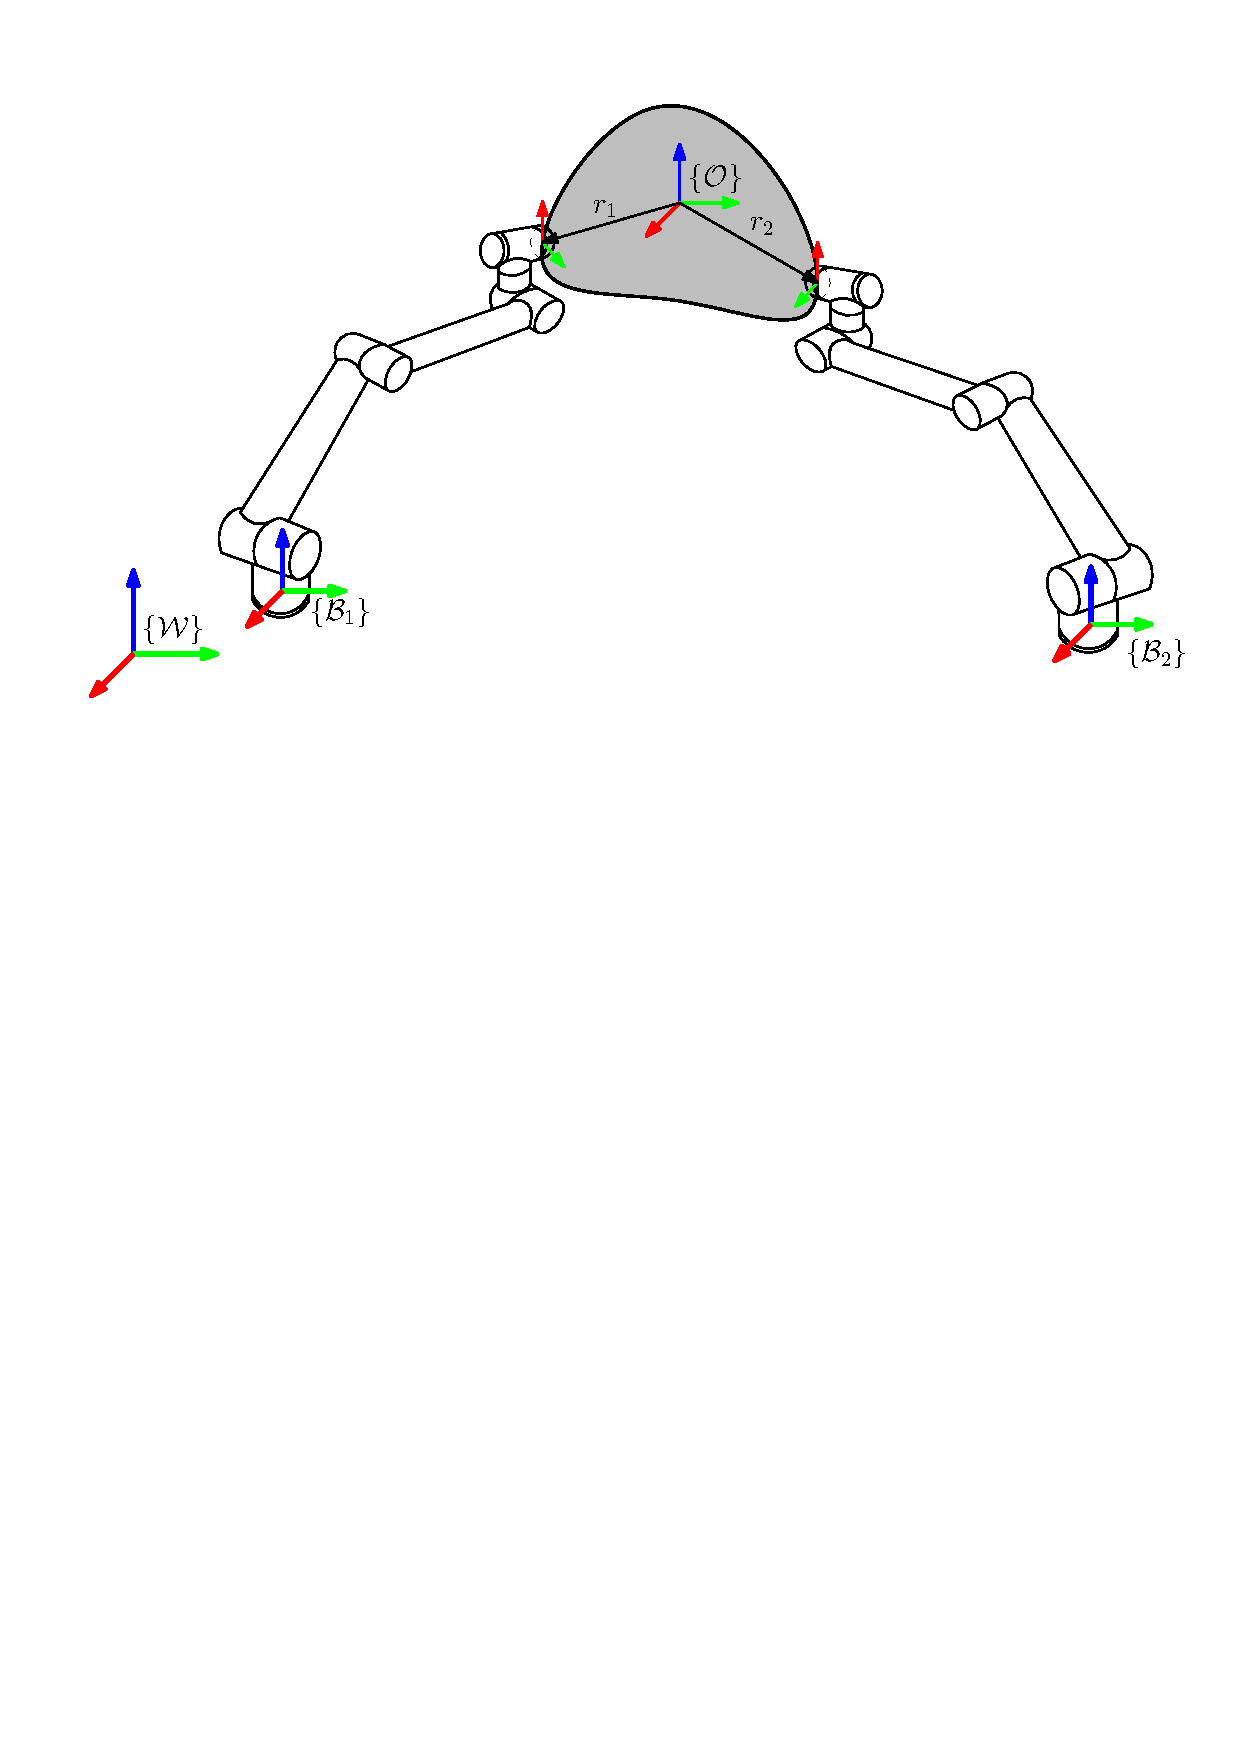
\includegraphics[width=\textwidth]{inc/img/object_coop_move}
  \caption{Кооперативная система, удерживающая объект манипулирования}
  \label{coop_obj_handle}
\end{figure}

Чаще всего объект манипулирования представляют абсолютно недеформируемым \cite{Schneider1989} или деформируемым по закону Гука \cite{Sun1996}. В общем случае модель объекта рассматривается, как модель абсолютно твердого тела:
\begin{equation}
        M_o(x_щ)\ddot{x}_o + C_o(x_o,\dot{x}_o)\dot{x}_o + g_o(x_o) =  f_o ,
        \label{eq:obj_base_model}
    \end{equation}
где $x_o \in \R_{6\times1}$ --- вектор положения и ориентации(углы Эйлера) объекта манипулирования, $f_o \in \R_{6\times1}$ --- силы/моменты, действующие на объекта со стороны манипуляторов, $M_o(x_0)$, $C_o(x_o,\dot{x}_o)$,$g_o(x_o)$ --- матрицы инерции, центробежных сил и гравитации соответственно объекта манипулирования.

Одними из первых алгоритмы силомоментного управления применили к управлению кооперативной системой манипуляционных роботов Р. Бонитц \cite{Bonitz1996} и С. Шнайдер \cite{Schneider1989}(импедансное управление) а также Т. Йошикава \cite{Yoshikawa1990}(гибридное позиционое/силомоментное управление). Эти и более современные методы базируются на разделении сил, на внутренние (контактные) и внешние. Внутренние силы $\lambda_c$ вызывают деформацию тела, но не приводят к его движению. Внешние силы $h_c$, напротив, способны совершать работу по перемещению манипулируемого объекта:
\begin{equation}
  F_c = \lambda_c + h_c, \qquad \quad F_c = \begin{bmatrix} f_{c,1} & \dots & f_{c,k} \end{bmatrix}^\top,
\end{equation}
где $f_{c,i}$ --- сила возникающая, на рабочем инструменте $i$-го манипулятора, $F_c$ --- вектор агрегированных сил кооперативной системы, $k$ --- колличество агентов в кооперативной системе.

Для определения вектора сил $f_o$, действующих на объект и вызывающих его перемещение, можно воспользоваться матрицей схватывания \cite{AzizZadeh2019}:
\begin{equation}
        f_o =  G \cdot F_c = G\cdot \begin{bmatrix} f_{c,1} \\ \vdots\\  f_{c,k}\end{bmatrix}, G = \begin{bmatrix} I_3& 0_3 & \dots &  I_3 & 0_3 \\ S(r_1) & I_3 & \dots &  S(r_k) & I_3\end{bmatrix},
        \label{eq:grasping_matrix}
\end{equation}
где $r_i$ --- вектор от центра масс до точки контакта рабочего инструмента $i$-го манипулятора в базовой системе координат, изображенный на рисунке \ref{coop_obj_handle_rasp}, $S(r_i)$ -- его кососимметричная матрица.

\begin{figure}[ht]
  \centering
  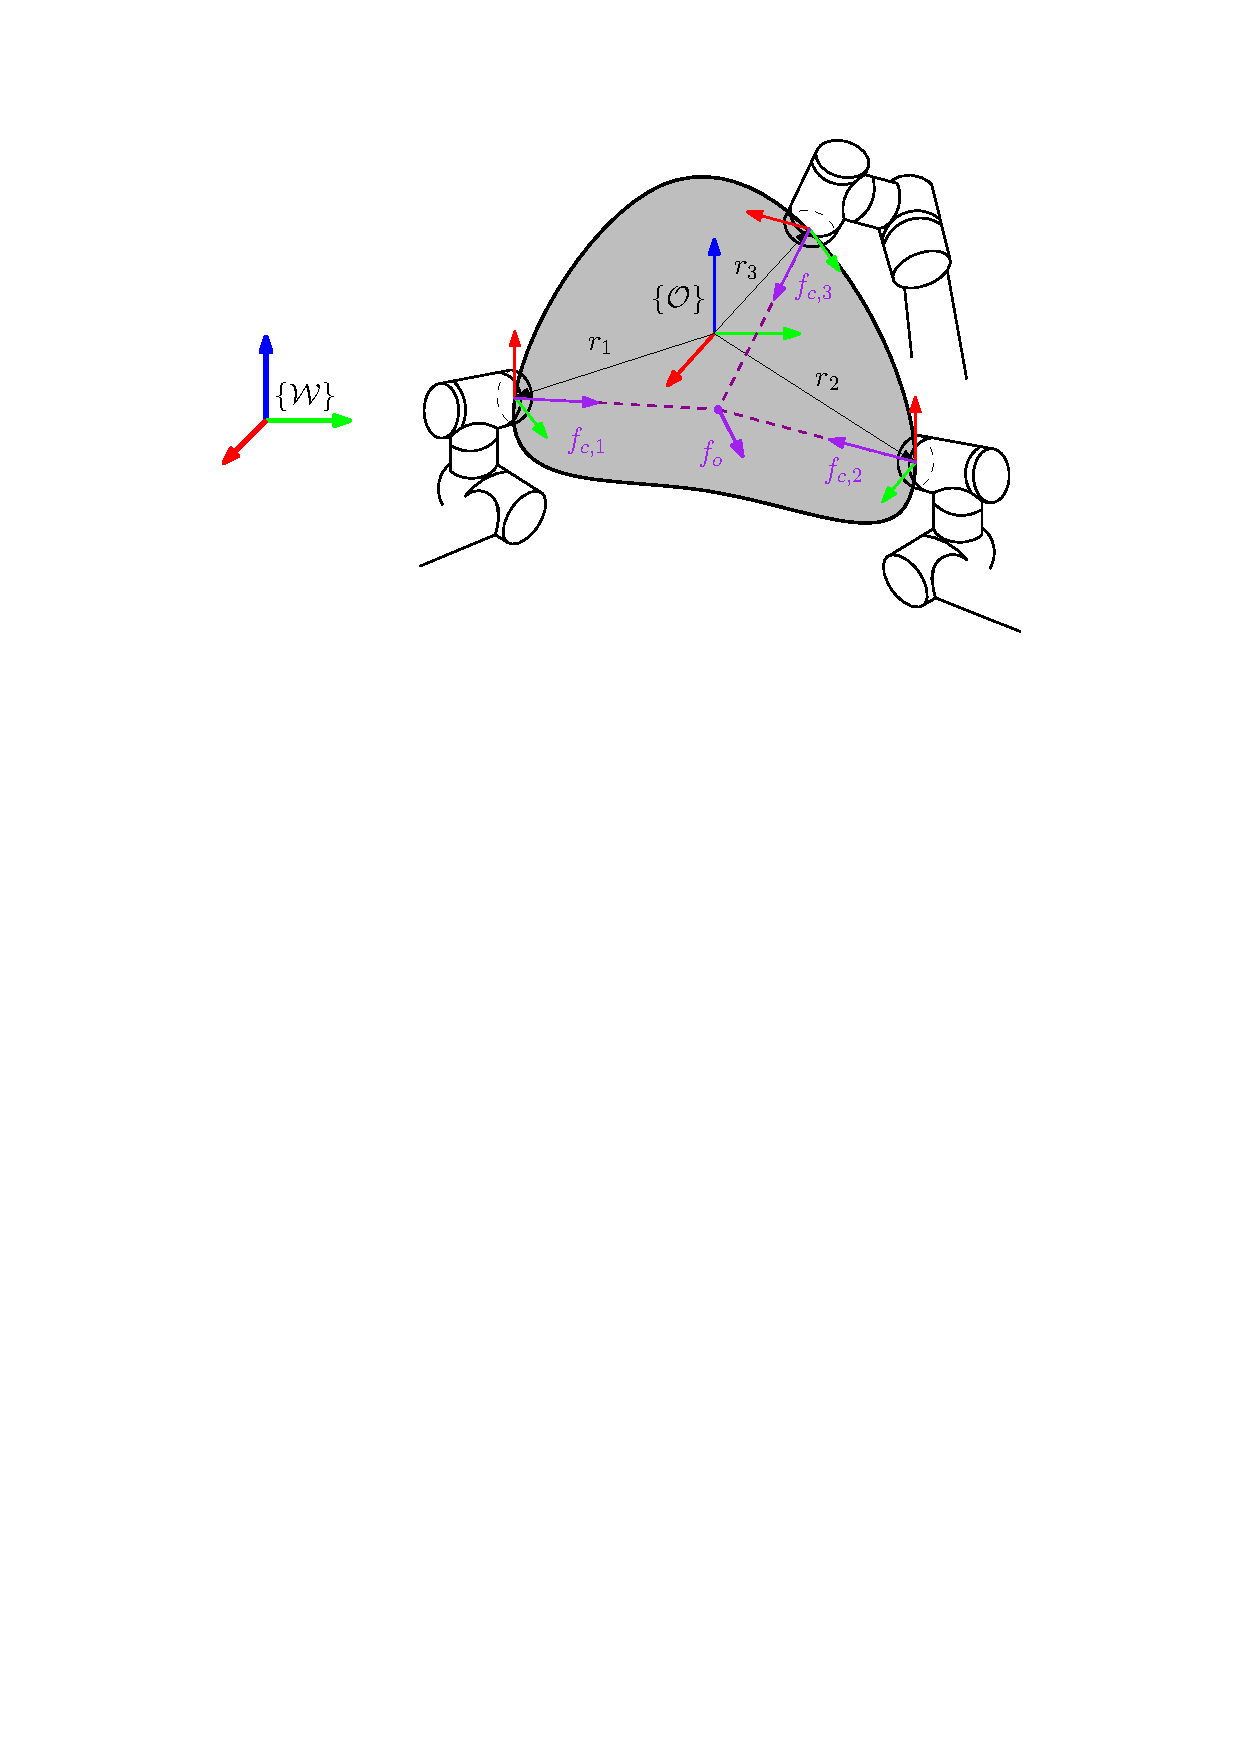
\includegraphics[width=0.65\textwidth]{inc/img/object_coop_internal_stress_rasp}
  \caption{Распределение сил в кооперативной системе}
  \label{coop_obj_handle_rasp}
\end{figure}

Из соотношения \eqref{eq:grasping_matrix} видно, что нельзя однозначно определить силы на рабочих инструментах манипуляторов $F_c =\begin{bmatrix} f_{c,1} & \dots & f_{c,k} \end{bmatrix}^\top$ из $f_o$ --- желаемых сил действующих на объект и перемещающих его. Наиболее простой и популярный подход --- использование псевдообращения:
\begin{equation}
  F_c = G^+ f_o
\end{equation}

Для разделения сил, на внутренние и внешние используют оператор проектирования $P$ на нуль пространство матрицы схватывания $G$ \cite{Lin2017}:
\begin{equation}
  \begin{cases}
    h_c = G^+G\cdot F_c,\\
    \lambda_c = P\cdot F_c, \quad P = (I - G^+G),
  \end{cases}
\end{equation}

Докажем, что силы $\lambda_c$ сосредоточены внутри объекта и определяют силу схватывания и деформации объекта, но не приводят к его движению:
        \begin{align}
            \text{Пусть}\quad F_c &= \lambda_c, \nonumber \\
            \text{Тогда}\quad  f_o &= GF_c = G\lambda_c  = G(I - G^+G)\lambda_c = (G - G)\lambda_c = 0 \nonumber \\
            \Rightarrow G\lambda_c &= 0
        \end{align}

Большинство современных работ, рассматривающих кооперативное управление манипуляционными роботами для удержания объекта, базируются на гибридном позиционном/силомоментном управлении. Так например в работе \cite{AzizZadeh2019} для описанных кинематических ограничений реализуется алгоритм  управления положением фрезерной установки и усилием, которое он создает, при фрезеровании. Однако в данном алгоритме для ассиптотического схождения ошибки управления к нулю необходимо знание динамических параметров и манипуляторов и удерживаемого объекта.

\begin{figure}[ht]
  \centering
  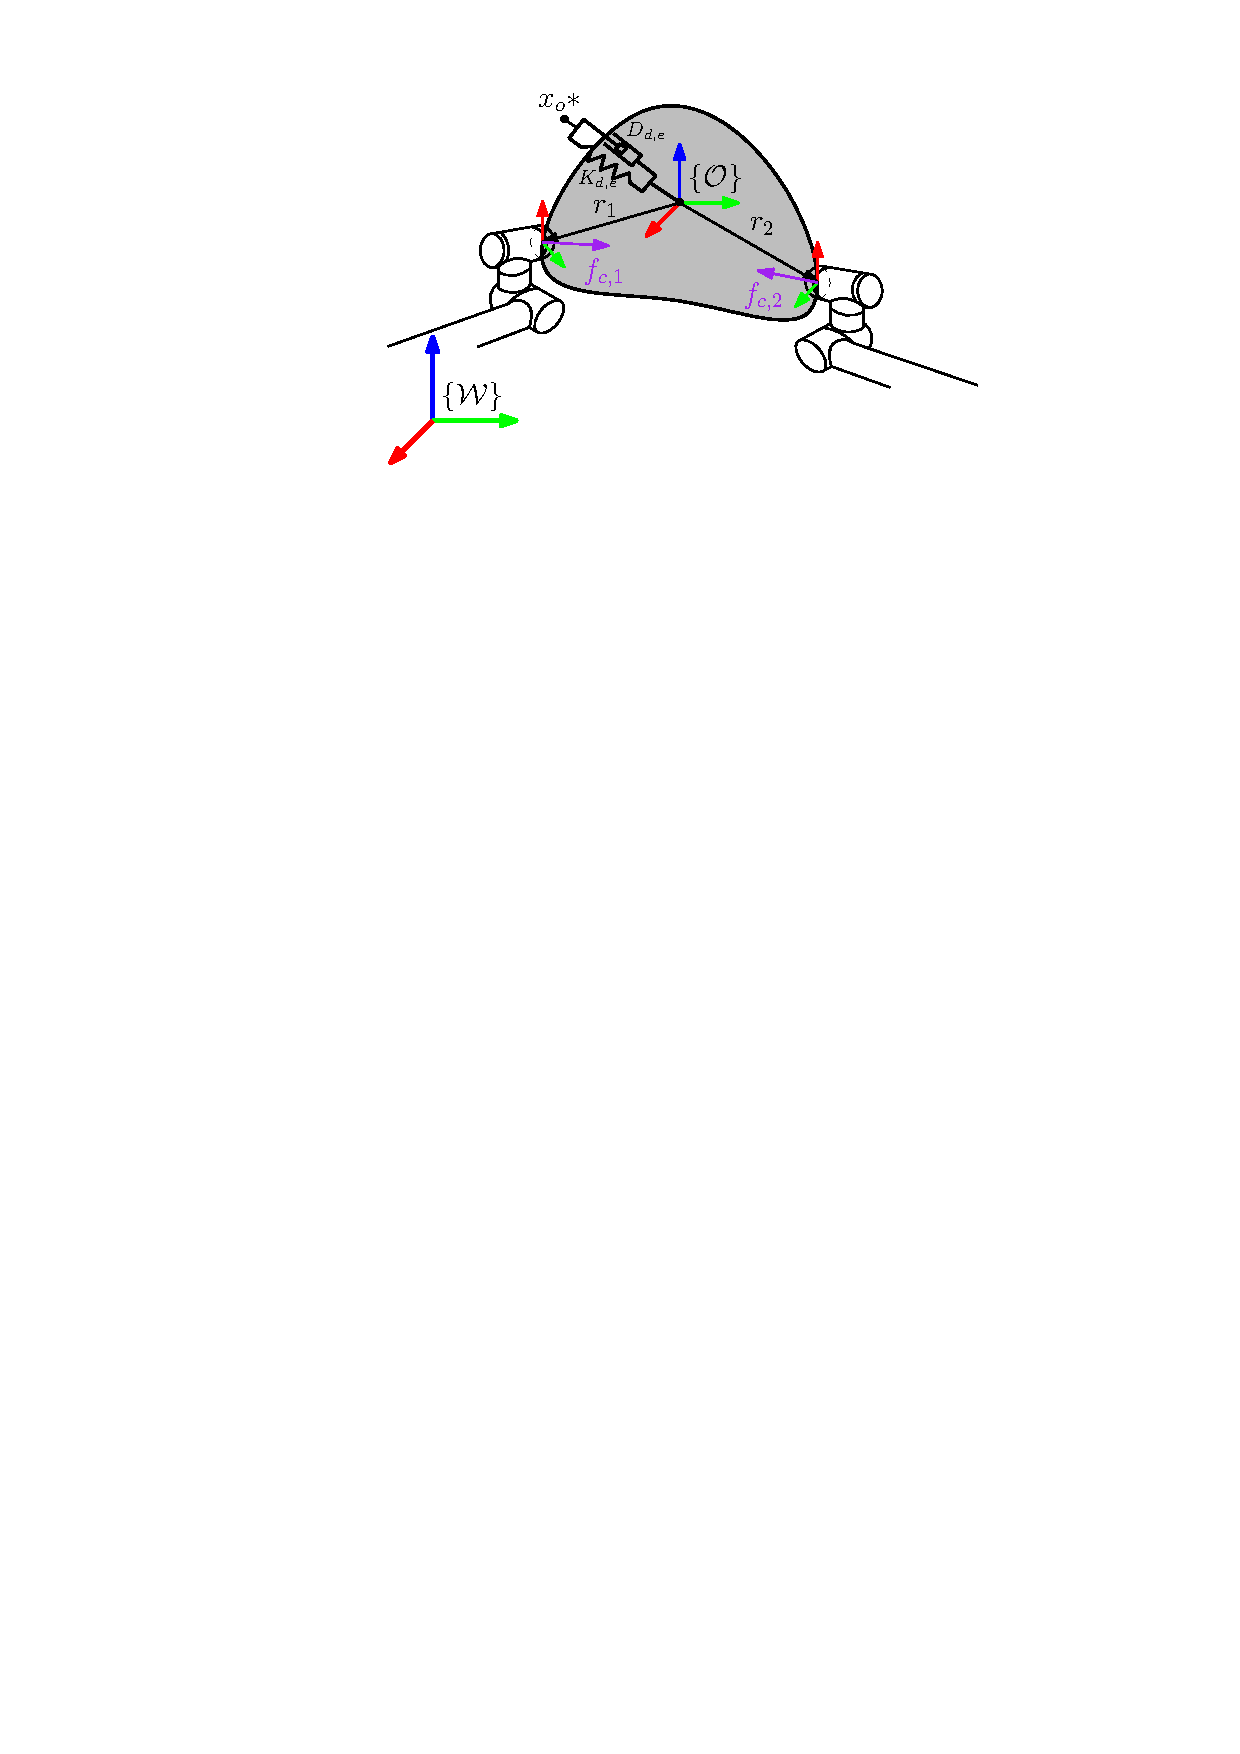
\includegraphics[width=0.65\textwidth]{inc/img/object_coop_internal_stress_global_impedance}
  \caption{Гибридное импедансное управление}
  \label{object_coop_internal_stress_global_impedance}
\end{figure}

В более давней работе \cite{Lin2017} информация об объекте не нужна, однако целью управления является поддержание заданного контактного усилия, что было реализовано с использованием все того же гибридного силомоментного управления. В данных алгоритмах необходимо априорное знание о расположении точек контакта манипуляторов с удерживаемым объектом. В более новой работе \cite{Jiao2020} представлен  упомянутый алгоритм гибридного импедансного управления(рисунок \ref{object_coop_internal_stress_global_impedance}), но адаптивный к изменению формы объекта манипулирования и расположению точек контакта. Однако, алгоритм неадаптивен к изменениям динамических параметров объекта манипулирования.
Предлагаемый в данной работе алгоритм в отличие от представленных адаптивен к параметрической неопределенности динамических параметров объекта манипулирования.




% \section{Анализ того и сего}
%
% % Обратите внимание, что включается не ../dia/..., а inc/dia/...
% % В Makefile есть соответствующее правило для inc/dia/*.pdf, которое
% % берет исходные файлы из ../dia в этом случае.
%
% \begin{figure}
%   \centering
%   \includegraphics[width=\textwidth]{inc/dia/rpz-idef0}
%   \caption{Рисунок}
%   \label{fig:fig01}
% \end{figure}
%
% \begin{figure}
%   \centering
%   \includegraphics[height=0.85\textheight]{inc/img/leonardo}
%   \caption{Предполагаемый автопортрет Леонардо да Винчи}
%   \label{fig:leonardo}
% \end{figure}
%
% В \cite{Pup09} указано, что...
%
% Кстати, про картинки. Во-первых, для фигур следует использовать \texttt{[ht]}. Если и после этого картинки вставляются <<не по ГОСТ>>, т.е. слишком далеко от места ссылки, "--- значит у вас в РПЗ \textbf{слишком мало текста}! Хотя и ужасный параметр \texttt{!ht} у окружения \texttt{figure} тоже никто не отменял, только при его использовании документ получается страшный, как в ворде, поэтому просьба так не делать по возможности.
%
% \section{Существующие подходы к созданию всячины}
%
% Известны следующие подходы...
%
% \begin{enumerate}
% \item Перечисление с номерами.
% \item Номера первого уровня. Да, ГОСТ требует именно так "--- сначала буквы, на втором уровне "--- цифры.
% Чуть ниже будет вариант <<нормальной>> нумерации и советы по её изменению.
% Да, мне так нравится: на первом уровне выравнивание элементов как у обычных абзацев. Проверим теперь вложенные списки.
% \begin{enumerate}
% \item Номера второго уровня.
% \item Номера второго уровня. Проверяем на длииииной-предлиииииииииинной строке, что получается.... Сойдёт.
% \end{enumerate}
% \item По мнению Лукьяненко, человеческий мозг старается подвести любую проблему к выбору
%   из трех вариантов.
% \item Четвёртый (и последний) элемент списка.
% \end{enumerate}
%
% Теперь мы покажем, как изменить нумерацию на «нормальную», если вам этого захочется. Пара команд в начале документа поможет нам.
%
% \renewcommand{\labelenumi}{\arabic{enumi})}
% \renewcommand{\labelenumii}{\asbuk{enumii})}
%
% \begin{enumerate}
% \item Изменим нумерацию на более привычную...
% \item ... нарушим этим гост.
% \begin{enumerate}
% \item Но, пожалуй, так лучше.
% \end{enumerate}
% \end{enumerate}
%
% В заключение покажем произвольные маркеры в списках. Для них нужен пакет \textbf{enumerate}.
% \begin{enumerate}[1.]
% \item Маркер с арабской цифрой и с точкой.
% \item Маркер с арабской цифрой и с точкой.
% \begin{enumerate}[I.]
% \item Римская цифра с точкой.
% \item Римская цифра с точкой.
% \end{enumerate}
% \end{enumerate}
%
% В отчётах могут быть и таблицы "--- см. табл.~\ref{tab:tabular} и~\ref{tab:longtable}.
% Небольшая таблица делается при помощи \Code{tabular} внутри \Code{table} (последний
% полностью аналогичен \Code{figure}, но добавляет другую подпись).
%
% \begin{table}[ht]
%   \caption{Пример короткой таблицы с коротким названием}
%   \begin{tabular}{|r|c|c|c|l|}
%   \hline
%   Тело      & $F$ & $V$  & $E$ & $F+V-E-2$ \\
%   \hline
%   Тетраэдр  & 4   & 4    & 6   & 0         \\
%   Куб       & 6   & 8    & 12  & 0         \\
%   Октаэдр   & 8   & 6    & 12  & 0         \\
%   Додекаэдр & 20  & 12   & 30  & 0         \\
%   Икосаэдр  & 12  & 20   & 30  & 0         \\
%   \hline
%   Эйлер     & 666 & 9000 & 42  & $+\infty$ \\
%   \hline
%   \end{tabular}
%   \label{tab:tabular}
% \end{table}
%
% Для больших таблиц следует использовать пакет \Code{longtable}, позволяющий создавать
% таблицы на несколько страниц по ГОСТ.
%
% Для того, чтобы длинный текст разбивался на много строк в пределах одной ячейки, надо в
% качестве ее формата задавать \texttt{p} и указывать явно ширину: в мм/дюймах
% (\texttt{110mm}), относительно ширины страницы (\texttt{0.22\textbackslash textwidth})
% и~т.п.
%
% Можно также использовать уменьшенный шрифт "--- но, пожалуйста, тогда уж во \textbf{всей}
% таблице сразу.
%
% \begin{center}
%   \begin{longtable}{|p{0.40\textwidth}|c|p{0.30\textwidth}|}
%     \caption{Пример длинной таблицы с длинным названием на много длинных-длинных строк}
%     \label{tab:longtable}
%     \\ \hline
%     Вид шума & Громкость, дБ & Комментарий \\
%     \hline \endfirsthead
%     \subcaption{Продолжение таблицы~\ref{tab:longtable}}
%     \\ \hline \endhead
%     \hline \subcaption{Продолжение на след. стр.}
%     \endfoot
%     \hline \endlastfoot
%     Порог слышимости             & 0     &                                                \\
%     \hline
%     Шепот в тихой библиотеке     & 30    &                                                \\
%     Обычный разговор             & 60-70 &                                                \\
%     Звонок телефона              & 80    & \small{Конечно, это было до эпохи мобильников} \\
%     Уличный шум                  & 85    & \small{(внутри машины)}                        \\
%     Гудок поезда                 & 90    &                                                \\
%     Шум электрички               & 95    &                                                \\
%     \hline
%     Порог здоровой нормы         & 90-95 & \small{Длительное пребывание на более
%     громком шуме может привести к ухудшению слуха}                                        \\
%     \hline
%     Мотоцикл                     & 100   &                                                \\
%     Power Mower                  & 107   & \small{(модель бензокосилки)}                  \\
%     Бензопила                    & 110   & \small{(Doom в целом вреден для здоровья)}     \\
%     Рок-концерт                  & 115   &                                                \\
%     \hline
%     Порог боли                   & 125   & \small{feel the pain}                          \\
%     \hline
%     Клепальный молоток           & 125   & \small{(автор сам не знает, что это)}          \\
%     \hline
%     Порог опасности              & 140   & \small{Даже кратковременное пребывание на
%     шуме большего уровня может привести к необратимым последствиям}                       \\
%     \hline
%     Реактивный двигатель         & 140   &                                                \\
%                                  & 180   & \small{Необратимое полное повреждение
%                                  слуховых органов}                                        \\
%     Самый громкий возможный звук & 194   & \small{Интересно, почему?..}                   \\
%   \end{longtable}
% \end{center}

%%% Local Variables:
%%% mode: latex
%%% TeX-master: "rpz"
%%% End:

\chapter{Математическое описание системы и постановка задачи}
\label{cha:design}

Для синтеза алгоритма управления кооперативной системы из двух артикулированных шестизвенных манипуляторов формализуем ее кинематической и динамической модели. Кинематика каждого манипулятора описывается в соответствии с соглашением Денавита – Хартенберга \cite{Spong2006}.
Обозначения для кинематических параметров артикулированного робота-манипулятора представлены на рисунке \ref{fig:dh_convention}.

\begin{figure}[ht!]
  \centering
  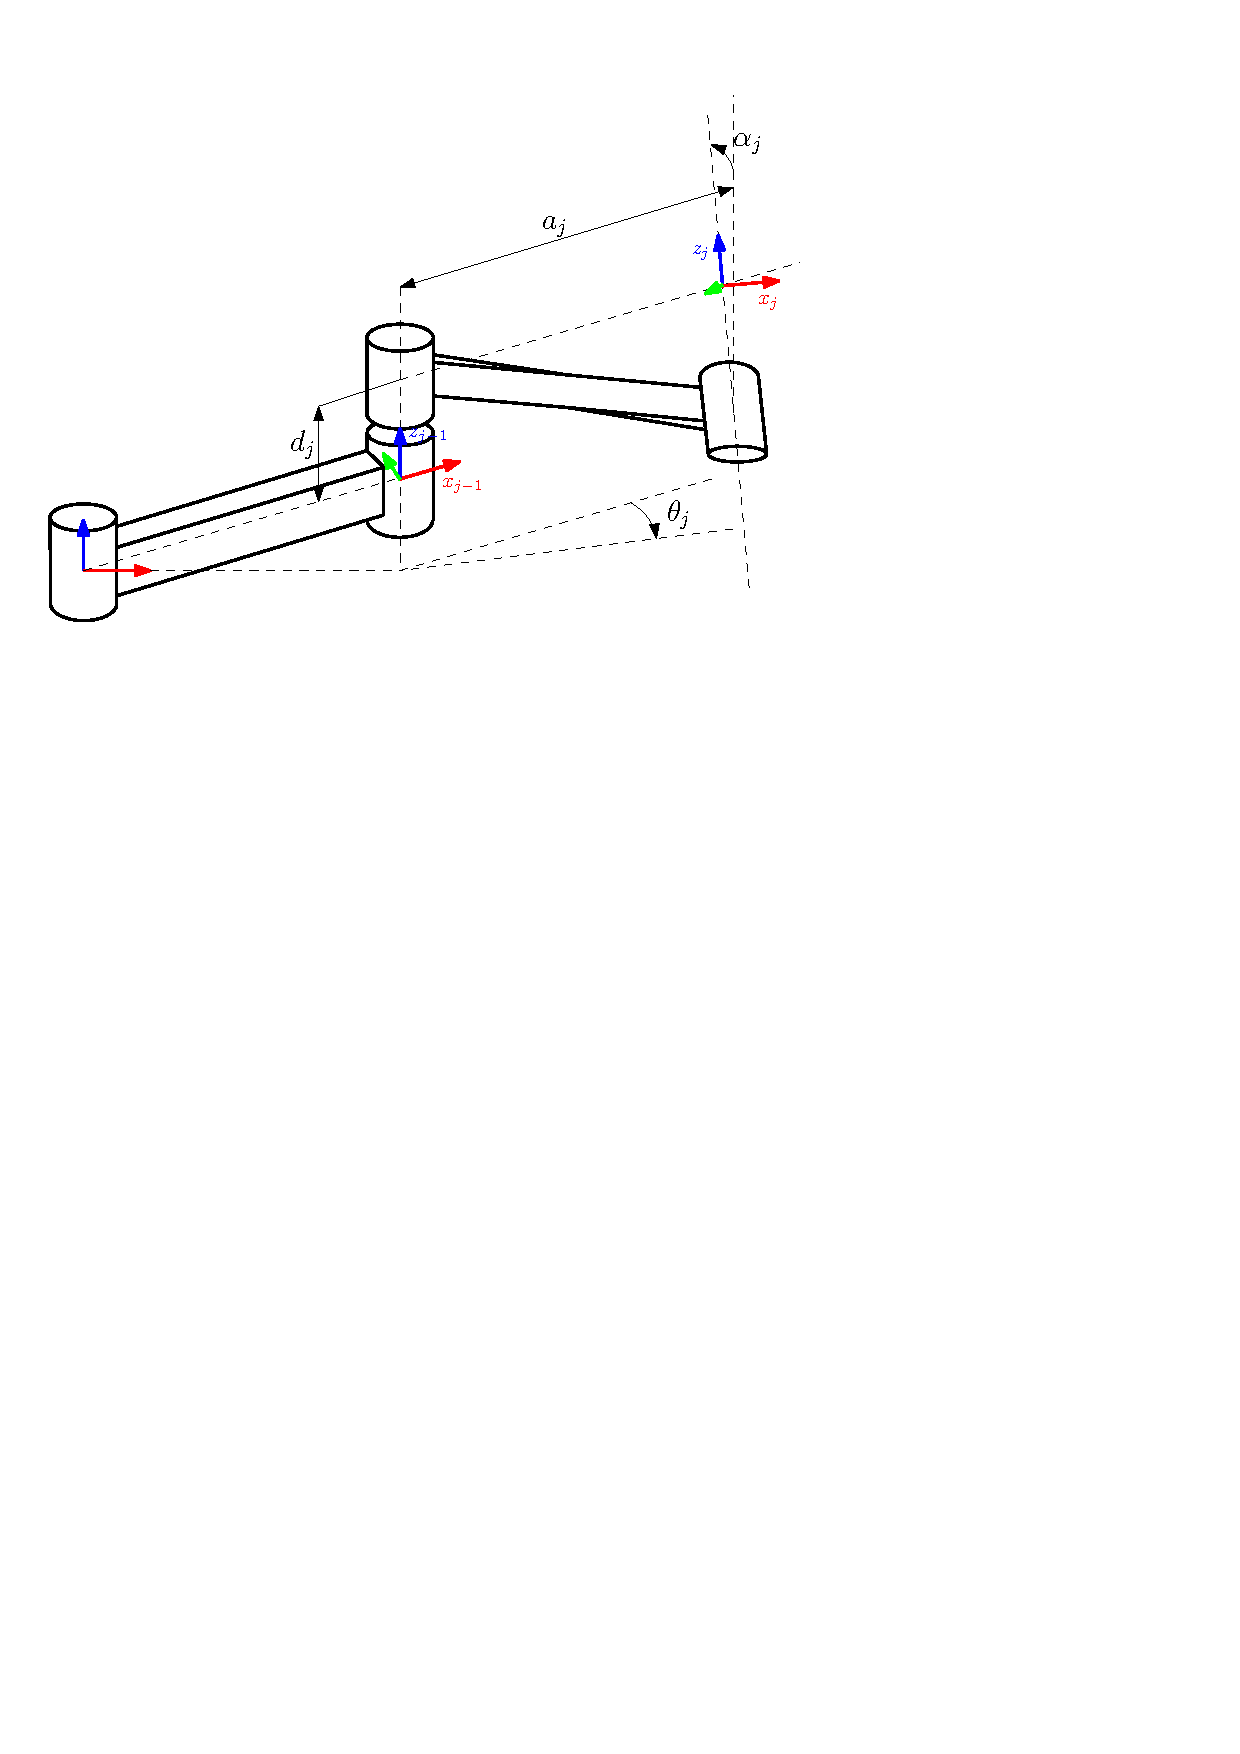
\includegraphics[width=0.7\textwidth]{inc/img/dh_convention}
  \caption{Описание параметров Денавита-Хартенберга}
  \label{fig:dh_convention}
\end{figure}

Для синтеза алгоритма кооперативного управления ограничимся рассмотрением кооперации двух артикулированных манипуляторов, т.е $k=2$. Осуществленный в последующем разделе синтез справедлив и для систем с большим числом агентов $k$. Стоит отметить, что полученный алгоритм требует модификации для управления избыточными манипуляторами.

\section{Кинематика кооперативной системы}
\label{coop_kin}
Координаты рабочего инструмента каждого манипулятора могут быть получены из решения прямой задачи кинематики:
\begin{equation}
  p_i(q_i) = \begin{bmatrix}  o_{6,i}(q_i) \\ \varphi_i(q_i) \end{bmatrix},\quad i = \overline{1,2}\ ,
\end{equation}
где $p_i \in \R_{6\times1}$ --- вектор состоящий из вектора координат $o_{6,i} \in \R_{3\times1}$ и ориентаций(углов Эйлера) $\varphi_i \in \R_{3\times1}$ рабочего инструмента $i$-го манипулятора в базовой системе координат, $q_i=\theta_i \in \R_{6\times 1}$ --- вектор угловых положений сочленений $i$-го манипулятора.\\

Для определения скорости движения объекта манипулирования введем понятие относительной матрицы Якоби $i$ - го манипулятора:
\begin{equation*}
      J_{r,i} = \begin{bmatrix} z_{0,i}\times(x_o - o_{0,i}) & \dots & z_{5,i}\times(x_o - o_{5,i})\\
      z_{0,i} & \dots & z_{5,i} \end{bmatrix},\quad i =\overline{1,2}
\end{equation*}
где $o_{j,i}$ --- вектор координат положения $j$-го сочленения $i$-го манипулятора в базовой системе координат,  $z_{j,i}$ --- орт-вектор оси вращения $j$-го сочленения $i$-го манипулятора, $\displaystyle x_o  = \begin{bmatrix}
  o_o \\ \varphi_o
\end{bmatrix} \in \R_{6\times 1}$ --- координаты и ориентация(углы Эйлера) объекта манипулирования.

В случае жесткого удерживания, т.е когда вектор от начала системы координат объекта, до точки рабочего инструмента постоянен: $r_i=const$, получим следующие кинематические ограничения:
\begin{equation}
   \begin{bmatrix} \upsilon_o \\ \omega_o \end{bmatrix} = J_{r,1}\cdot \dot{q}_1 = J_{r,2}\cdot \dot{q}_2
\end{equation}

Так как измерение положения объекта манипулирования не представляется нам возможным,то примем наиболее часто используемое допущение \cite{Handbook}, что:
\begin{equation}
  x_o = \frac{1}{2}(p_1 + p_2),\quad \begin{bmatrix} \upsilon_o \\ \omega_o \end{bmatrix} = \begin{bmatrix} \frac{1}{2}J_1 & \frac{1}{2}J_2\end{bmatrix}\cdot \dot{q}_c = J_o \cdot \dot{q}_c, \quad q_c = \begin{bmatrix} q_1 \\ q_2\end{bmatrix}
\end{equation}
Стоит отметить также взаимосвязь между вектором $\dot{x}_o$ содержащем производной вектора углов Эйлера и вектором $\begin{bmatrix} \upsilon_o \\ \omega_o \end{bmatrix}$, содержащим значение скоростей вращения вокруг осей $x$, $y$, и $z$ в базовой системе координат:
\begin{equation}
  \quad \dot{x_o} = T_a^{-1} \begin{bmatrix} \upsilon_o \\ \omega_o \end{bmatrix}
\end{equation}
\section{Динамика кооперативной системы}
\label{coop_dyn}
Динамика каждого манипулятора, описывается уравнением \eqref{eq:base_one_manipulator_model} с соответствующим индексом для $i$-го манипулятора:
\begin{equation}
  M_i(q_i)\ddot{q}_i + C_i(q_i,\dot{q}_i)\dot{q}_i + g_i(q_i) = \tau_{c,i} - J_i^\top(q_i) f_{c,i}, \quad i =\overline{1,2} \ ,
  \label{eq:base_i_manipulator_model}
\end{equation}

Для упрощения изложения введем агрегирование векторов и матриц моментов и сил на рабочих инструментах:
\begin{equation}
   J_c = \begin{bmatrix} J_1(q_1) & 0_6\\ 0_6 & J_2(q_2) \end{bmatrix},\quad  \tau_c = \begin{bmatrix} \tau_{c,1}\\ \tau_{c,2} \end{bmatrix} = J_c^\top \cdot F_c
\end{equation}

Распишем более подробно динамическую модель объекта манипулирования, которая в общем виде задана уравнением \ref{eq:obj_base_model}.
Кинетическая энергия объекта манипулирования по теореме Кёнига состоит из кинетической энергии его поступательного и вращательного движения:
\begin{equation}
  K = \frac{1}{2}m_o\cdot \upsilon^\top_o \upsilon_o + \frac{1}{2} \omega_o^\top R I_o R^\top \omega_o
\end{equation}


\section{Постановка задачи}
Для заданной в предыдущих пунктах \ref{coop_kin} и \ref{coop_dyn} кооперативной системы из двух артикулированных роботов-манипуляторов синтезировать алгоритм гибридного позиционного/силомоментного управления для удержания объекта в заданном положении с желаемым контактным усилием при условии отсутствии знаний динамических параметров объекта манипулирования.

%
%
% \paragraph{Проверка} параграфа. Вроде работает.
% \paragraph{Вторая проверка} параграфа. Опять работает.
%
% Вот.
%
% \begin{itemize}
% \item Это список с <<палочками>>.
% \item Хотя он и по ГОСТ, но\dots
% \end{itemize}
%
% \begin{enumerate}
% \item  Для списка, начинающегося с заглавной буквы, лучше список с цифрами.
% \end{enumerate}
%
% Формула \eqref{F:F1} совершено бессмысленна.
%
% %Кстати, при каких-то условиях <<удавалось>> получить двойный скобки вокруг номеров формул. Вопрос исследуется.
%
% \begin{equation}
% a= cb
% \label{F:F1}
% \end{equation}
%
% А формула~\eqref{eq:fourierrow} имеет некоторый смысл.
% Кроме этого она пытается иллюстрировать применение окружения \Code{eqndesc} которое размещает формулу совместно с её описанием.
% Однако обратите внимание на нумерацию формул~\eqref{eq:fourierrow} и \eqref{F:F2}, попробуйте добавить \Code{[H]} к такой формуле.
%
% \begin{eqndesc}
%     \begin{equation}\label{eq:fourierrow}
%         f(x) = \frac{a_0}{2} + \sum\limits_{k=1}^{+\infty} A_k\cos\left(k\frac{2\pi}{\tau}x+\theta_k\right)
%     \end{equation}
%
%     где $A_k$ "--- амплитуда  k-го гармонического колебания,\\
%     $A_k$ "--- амплитуда $k$-го гармонического колебания,\\
%     $ k\frac{2\pi}{\tau} = k\omega$ "--- круговая частота гармонического колебания,\\
%     $\theta_k$ "--- начальная фаза $k$-го колебания.
% \end{eqndesc}
%
%
% Окружение \texttt{cases} опять работает (см. \eqref{F:F2}), спасибо И. Короткову за исправления..
%
%
% \begin{equation}
% a= \begin{cases}
%  3x + 5y + z, \mbox{если хорошо} \\
%  7x - 2y + 4z, \mbox{если плохо}\\
%  -6x + 3y + 2z, \mbox{если совсем плохо}
% \end{cases}
% \label{F:F2}
% \end{equation}
%
% \section{Подсистема всякой ерунды}
%
% Культурная вставка dot-файлов через утилиту dot2tex (рис.~\ref{fig:fig02}).
%
% \begin{figure}
%   \centering
% % [width=0.5\textwidth] --- регулировка ширины картинки
%   \includegraphics[width=.5\textwidth]{inc/dot/cow2}
%   \caption{Рисунок}
%   \label{fig:fig02}
% \end{figure}
%
%
% \subsection{Блок-схема всякой ерунды}
%
% \subsubsection*{Кстати о заголовках}
%
% У нас есть и \Code{subsubsection}. Только лучше её не нумеровать.

%%% Local Variables:
%%% mode: latex
%%% TeX-master: "rpz"
%%% End:

% \include{40-impl}
% \include{50-research}
% \include{60-economics}
% \include{70-bzd}

\backmatter %% Здесь заканчивается нумерованная часть документа и начинаются ссылки и

% \include{80-conclusion}%% заключение


\include{81-biblio}


\appendix   % Тут идут приложения

\include{90-appendix1}

\include{91-appendix2}

\end{document}

%%% Local Variables:
%%% mode: latex
%%% TeX-master: t
%%% End:
